\documentclass{mcmthesis}
\mcmsetup{CTeX = false,
    tcn = {12833},  %% your team control number
    problem = {B}, %% your chosen problem (A or B)
    sheet = true,
    titleinsheet = True,
    keywordsinsheet = true,
    titlepage = false,
    abstract = false}

\usepackage{newtxtext}%\usepackage{palatino}
\usepackage{comment}
\usepackage{lipsum}
\hypersetup{
    colorlinks=false,
    linkcolor=blue,
    filecolor=blue,
    urlcolor=blue,
    citecolor=cyan,
}
\usepackage{color}
\usepackage{float}
\numberwithin{figure}{section}
\numberwithin{table}{section}
\numberwithin{equation}{section}
\usepackage{enumerate}

\usepackage{placeins}
\usepackage{graphicx}
\usepackage[figuresright]{rotating}
\usepackage[final]{pdfpages}
%\usepackage[
%    backend=bibtex,
%    style=numeric-verb,
%]{biblatex}
\usepackage{babel}

%\addbibresource{citations.bib}


\title{CO\textsubscript{2} and Global Warming}

%! suppress = LineBreak
\begin{document}
\graphicspath{ {./images/} }
    \begin{abstract}
        Abstract

        \begin{keywords}
            Keywords, More Keywords
        \end{keywords}

    \end{abstract}

    \maketitle
    \tableofcontents
    \newpage 


    \section{Introduction}

    \subsection{Background}
    The most significant greenhouse gas on Earth is carbon dioxide, which both absorbs and radiates heat. In contrast to oxygen and nitrogen, which together make up the majority of our atmosphere, greenhouse gases absorb heat emitted from the Earth's surface and re-emit it in all directions, including back toward the planet's surface. The natural greenhouse effect that keeps the Earth's atmosphere above freezing would be insufficient without carbon dioxide. People are accelerating the natural greenhouse effect and raising the earth's temperature by releasing more carbon dioxide into the atmosphere. The NOAA Global Monitoring Lab found that in 2021, carbon dioxide accounted for nearly two thirds of the total heating influence of all greenhouse gases created by humans.

    Prior to the Industrial Revolution, carbon dioxide in the atmosphere was consistently around 280 parts per million (ppm).
    The concentration of CO\textsubscript{2} in the atmosphere reached 377.7 ppm
    in March 2004, resulting in the largest 10-year average
    increase up to that time. According to scientists from National
    Oceanographic and Atmospheric Administration (NOAA) and
    Scripps Institution of Oceanography (SIO) the monthly mean
    CO\textsubscript{2} concentration level peaked at 421 ppm in May 2022. An
    Organisation for Economic Co-Operations and Development
    (OECD) report predicts a CO\textsubscript{2} level of 685 ppm by 2050.


    \subsection{Problem Analysis}
    Our thought process and plan is presented here below as a flowchart:
    \begin{center}
        \frame{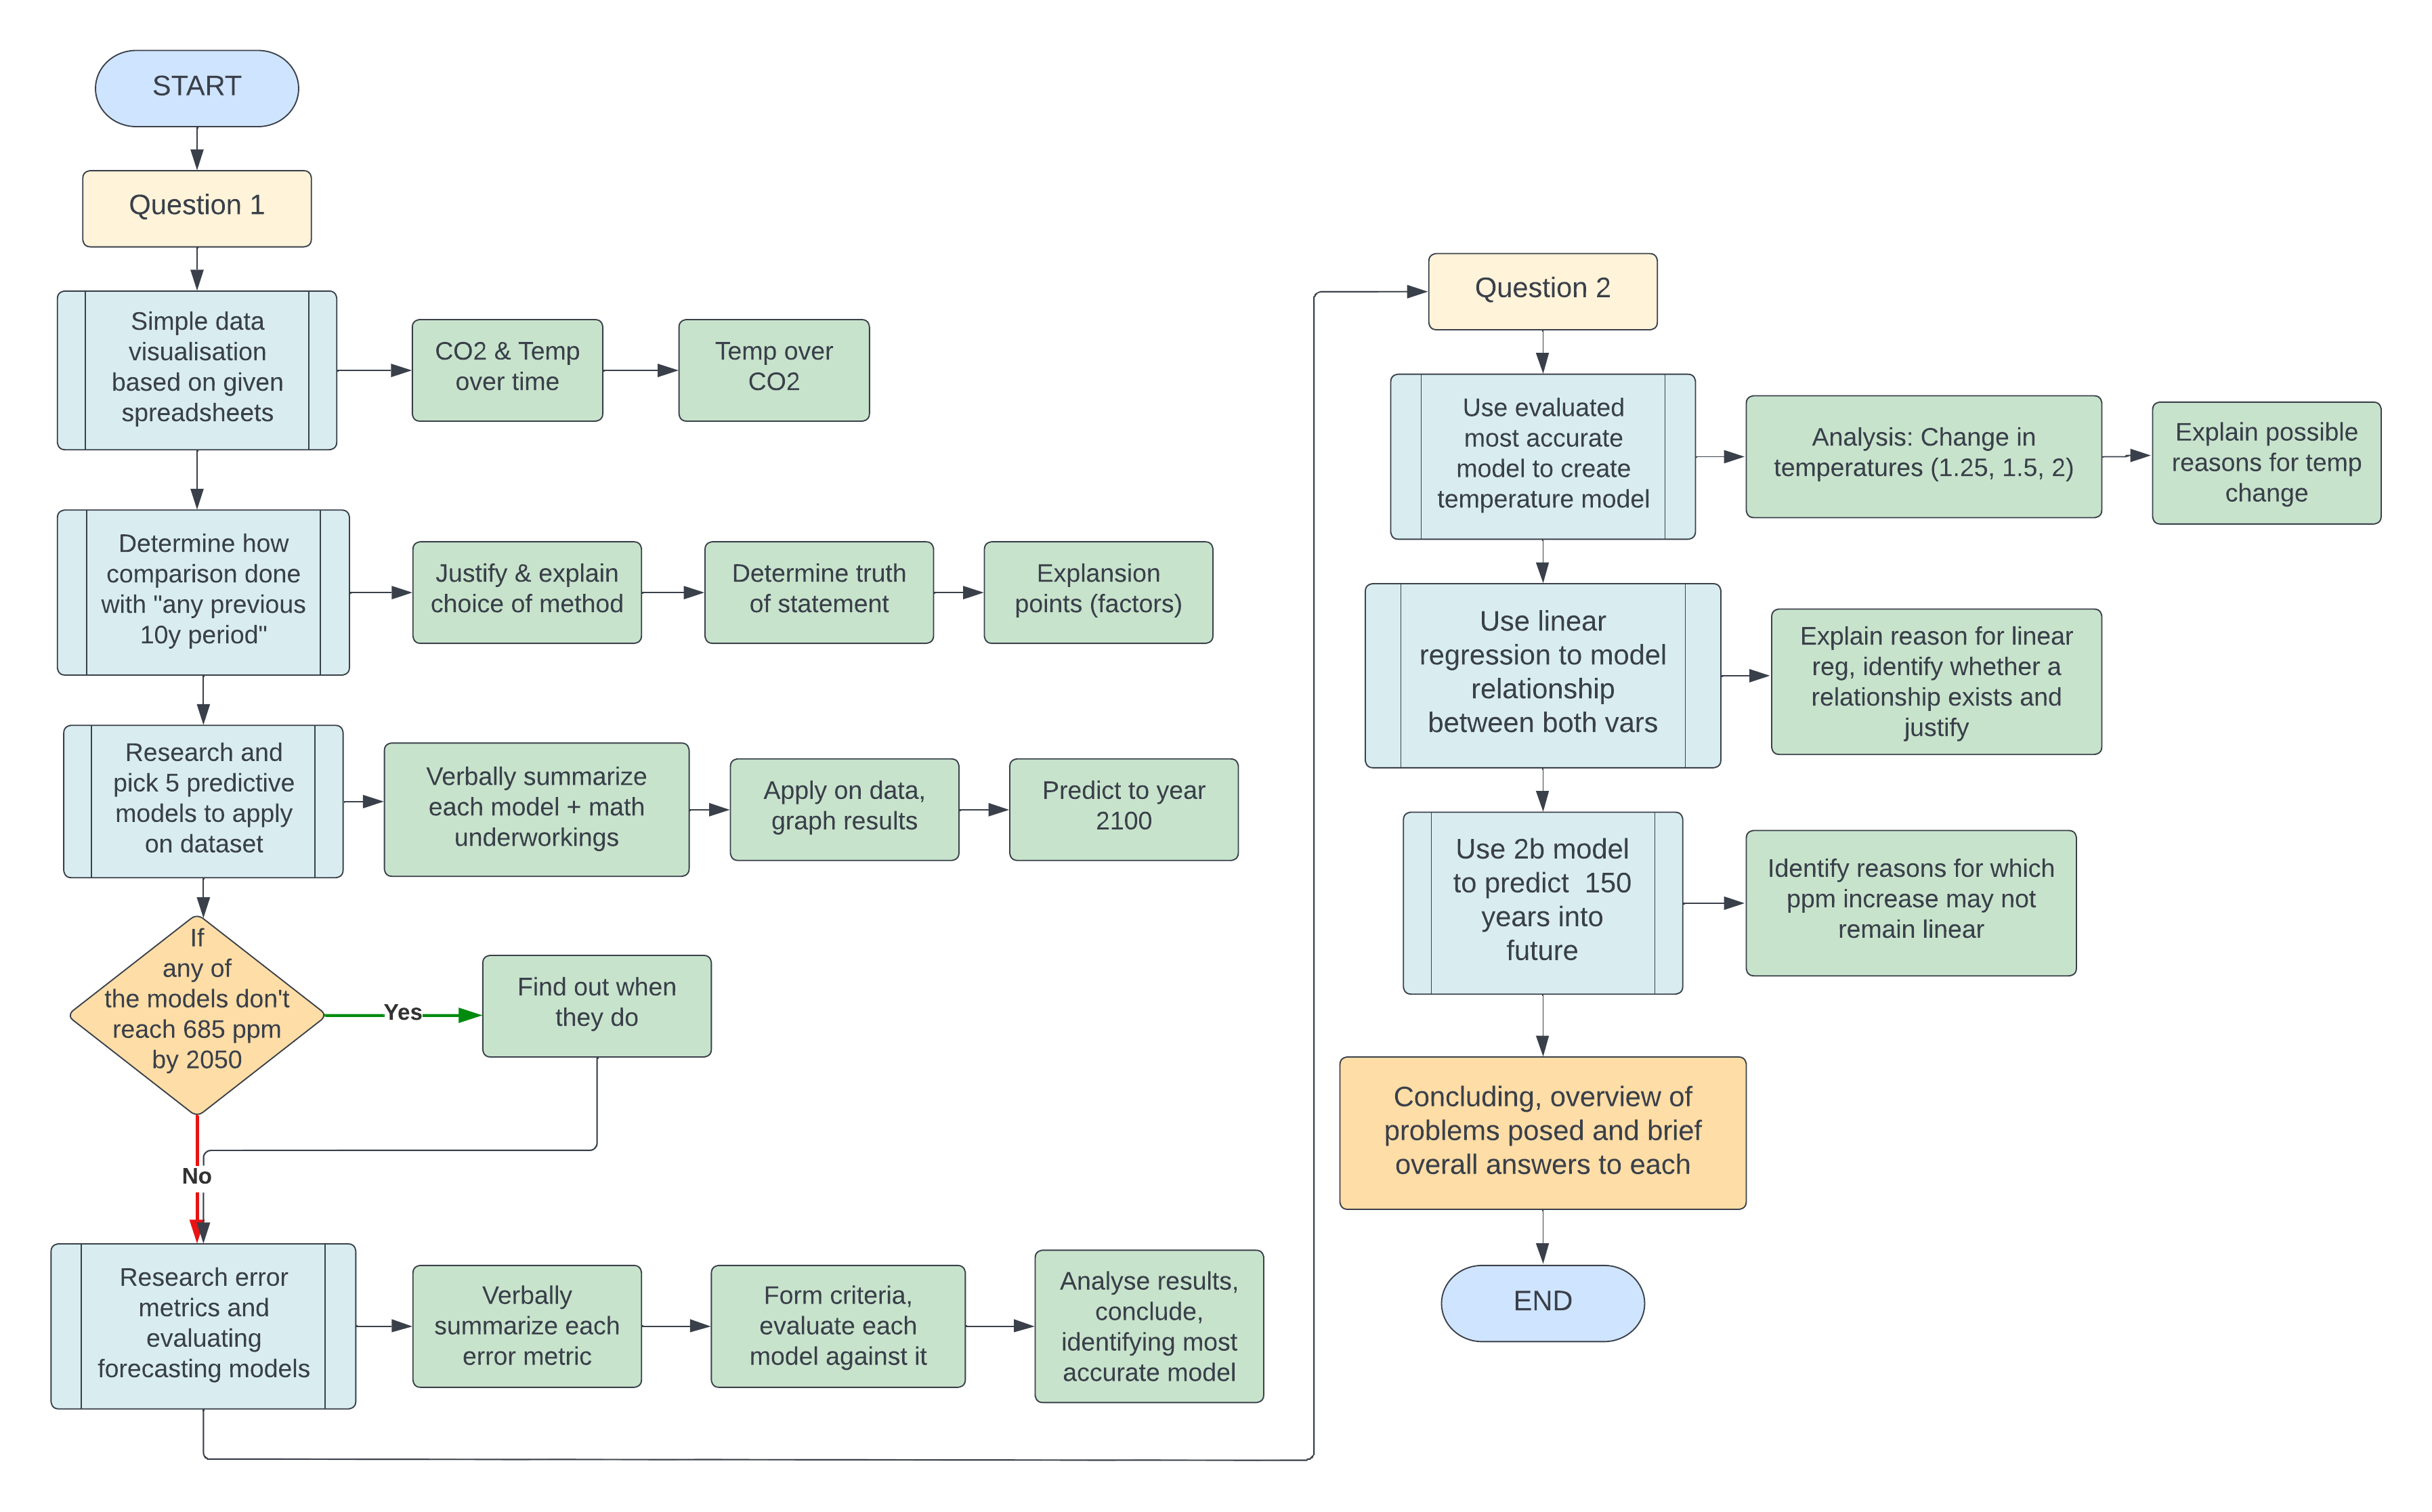
\includegraphics[scale=0.5]{plan}}
    \end{center}

    \noindent\textbf{Problem one}: Specifics

    \noindent\textbf{Problem two}: Specifics

    \subsection{Keyword Definitions}
    \noindent\textbf{Term 1}: Definition

    \noindent\textbf{Term 2}: Definition

    \noindent\textbf{Term 3}: Definition

    \subsection{Assumptions and Justifications}
    \noindent\textbf{Assumption 1}: Statement
    \textbf{Justification}: blah blah

    \noindent\textbf{Assumption 2}: Statement
    \textbf{Justification}: blah blah

    \noindent\textbf{Assumption 3}: Statement
    \textbf{Justification}: blah blah


    \section{Modeling}
    This is a general overview of the most appropriate mathematical models we can use to describe and predict data in relation to the problem. 



    \subsection{Variables and Parameters}
    See table 2.1:
    \begin{table}[h!]
        \centering
        \begin{tabular}{cc}
            \toprule
            Variable & Definition      \\
            \midrule
            $x$      & description     \\
            $y$      & description     \\
            $z$      & description     \\
            \bottomrule
        \end{tabular}
        \caption{Variables in the Model}
        \label{tab:my_label}
    \end{table}

    \subsection{Linear Regression}
    Linear regression is an approach used to model the linear relationship between an independent variable (x) and dependent variable (y), by fitting a linear equation. It is used to present the past values and predict others, in this case future CO\textsubscript{2} emissions. One of the most common and simplest methods used to obtain a regression line is the Ordinary Least Square (OLS) method. It involves minimizing the sum of the offsets of residuals of points from a plotted line, to then obtain the regression line. 

    To perform the method, a difference is first set between the dependent variable (CO\textsubscript{2}) and its estimation: ${(y - \hat{y})}$. The difference is then squared, and a summation taken for the entire data set: ${\displaystyle S = \sum (y - \hat{y}^2)}$. To obtain the parameters that make the sum of square difference become minimum, a partial derivative is taken for each parameter, then equated to 0: $${\displaystyle \frac{d S}{d \alpha} = 0}$$. The final formula for OLS that is obtained is denoted as:
    
    ${S = \sum{(y - \hat{y})^2} = \sum{(y - ax - b)^2}}$
    
    The formula was applied to the given data set to obtain the following line equation:
    
    ${y = 1.6140361 x - 2854.59326421}$
    
    {y} was then set to 685 to find the year at which CO\textsubscript{2} emissions would reach 685ppm; it was found that it would reach this level at the year 2193. The regression line was then graphed and used to predict the next 30 years of CO\textsubscript{2} emissions, the actual data was also plotted for comparison:

    \begin{center}
        \frame{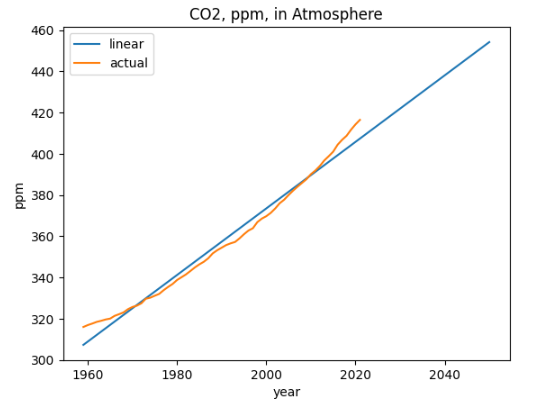
\includegraphics[scale=0.75]{linear}}
    \end{center}
    
    Linear regression is useful in relation to the problem as it is simple to interpret and portray, allowing the prediction of data to be accurate during interpolation. However, if the data to be predicted is outside of the range, such as predicting future CO\textsubscript{2} levels, extrapolation may be inaccurate due to a false assumption of the trend. Furthermore, if the variables plotted provide a non-linear relationship, a linear regression line may inaccurately represent and predict values, which is the case in the data provided.


    \subsection{Exponential Regression}
    The second approach decided upon was exponential regression, which models the non-linear relationship between an independent variable (x) and dependent variable (y). This choice was made based on visual indicators of the data given’s trend, exhibiting a possible exponential curve. The regression curve portrays data rapidly increasing; at an exponential rate. In exponential regression, the correlation can be denoted as:

    ${log(y) = log (A) + B t}$
    
    An exponential function contains a base and an exponent where: ${y = a b ^x}$. This function was then applied to the given data set to form the equation: ${y = 1.005717^(2.8427x - 4854.4) + 256.024}$. {y} was then set to 685 to find the year at which CO\textsubscript{2} emissions would reach 685ppm; it was found that it would reach this level at the year 2079. The equation was graphed alongside the actual values and linear regression line for comparison: 

    \begin{center}
        \frame{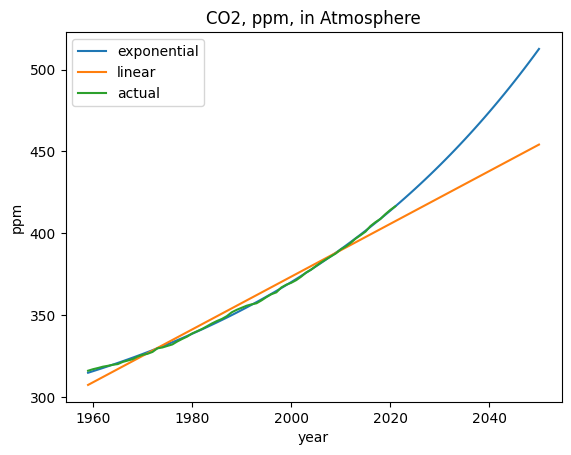
\includegraphics[scale=0.6]{exponential}}
    \end{center}

    Visually, the exponential function better aligns with the actual values; the predicted values also seem to fit with the general trend. An advantage of exponential regression as a predictive model is that it provides high quality forecasts, which increase the accuracy of predicted values during interpolation. However, a key drawback is that a large data set is necessary to carry this method out, as a reasonable amount of continuity is needed to accurately predict future values, especially during extrapolation.

    \subsection{Logistic Regression}
    The third predictive model selected shares similarities with the exponential model. One key difference however is that an exponential curve is J-shaped, whereas a logistic curve is sigmoid, the growth rate of the y-variable (CO\textsubscript{2}) increases during its lag phase, and eventually reaches a stationary phase. The logistic function has the equation:

    ${\displaystyle f(x)={\frac {L}{1+e^{-k(x-x_{0})}}}}$
    
    Where:
    \begin{itemize}
        \item {L} = Curve’s maximum value
        \item {k} = Logistic growth rate
        \item ${x_0}$ = X value of the sigmoid point
        \item {x} = Real number
    \end{itemize}
    
    The function’s parameters were then manually adjusted to best suit the current data set, giving the following equation: ${y = 2523.6 / (1 + e^{(-0.017587 * (x - 2175.5))}) + 260.0180641636529}$. {y} was then set to 685 to find the year at which CO\textsubscript{2} emissions would reach 685ppm, it was found that it would reach this level at the year 2193. The equation was then graphed alongside with the regression lines of the two previous models to obtain the following graph:

    \begin{center}
        \frame{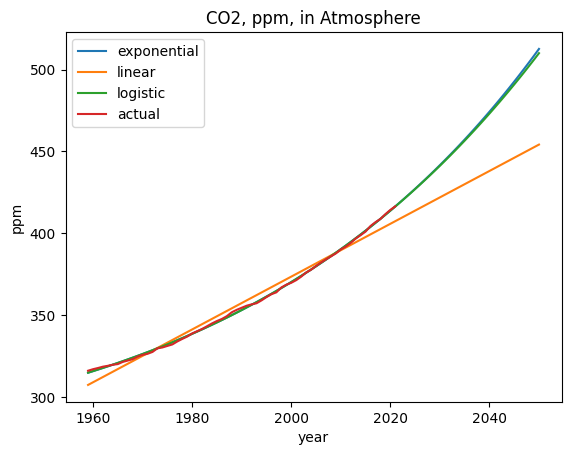
\includegraphics[scale=0.6]{logistic_2040}}
    \end{center}

    As can be seen, the logistic curve follows a very similar path to that of the exponential function. However, the 1959-2050 year range is too small to depict the sigmoid point, so the functions were graphed to reach the year 2400:

    \begin{center}
        \frame{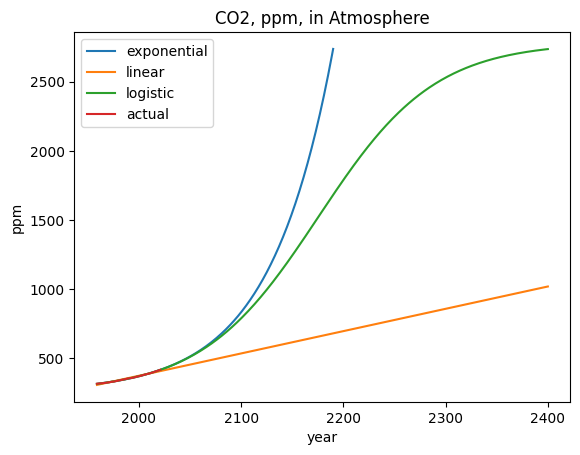
\includegraphics[scale=0.6]{logistic_2400}}
    \end{center}

    \subsection{Prophet}
    Prophet is a non-linear regression model released by Facebook, it is a procedure for forecasting time series data, working best with series that have strong seasonal effects of historical data. The graph for CO\textsubscript{2} levels over time can be plotted. The regression model is in the form: 

    ${\displaystyle y_t = g_t + s_t + h_t +\epsilon_t}$
    
    Where: 
    \begin{itemize}
        \item ${g_t}$ = Piecewise-linear trend
        \item ${s_t}$ = Seasonal patterns
        \item ${h_t}$ = Holiday effects
        \item ${\epsilon_t}$ = White noise error
    \end{itemize}

    \begin{center}
        \frame{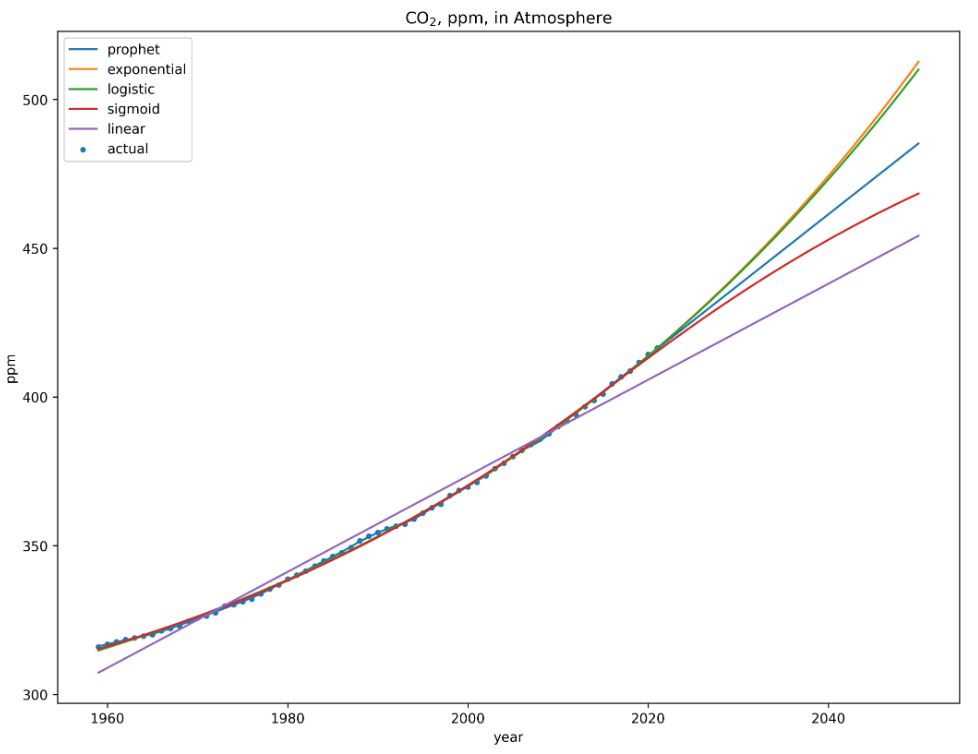
\includegraphics[scale=0.5]{prophet}}
    \end{center}

    Prophet is fast and generally maintains a high accuracy when predicting values. It can be used in a range of different contexts and it is robust to outliers, shifts in the overall trend and missing data.  A key disadvantage is that a larger set of data is needed to accurately depict a trend-line.

    \subsection{ARIMA Model}
    An additional time-series prediction model that was investigated was ARIMA, which is based on ARMA (AutoRegressive Moving Average). These models are widely used in datasets that demonstrate non-stationarity, where the series’ statistical properties such as mean, variance and autocorrelation change over time. ARIMA assumes the input data to be stationary, so any non-stationary data has to be made stationary through a reversible process. Usually, the transformation involves finding the general trend with methods such as regression and then using differencing to remove the trend from the dataset. With the trend eliminated, an ARIMA model can then be constructed and its optimal parameters found. 

    Another appropriate model to use in regards to  the data set is ARIMA. ARIMA models are generally denoted as ARIMA (p, d, q) where:
    \begin{itemize}
        \item p = Number of Auto-Regressive (AR) terms 
        \item d = Number of differencing
        \item q = Number of Moving Average (MA) terms
    \end{itemize}
    
    The functions AR(p) and MA(q) are defined below as:
    
    -----------THERES SUPPOSED TO BE A TABLE HERE----------

    Before tuning the parameters p and q, the number of differencing required to make the data stationary must be found out. To evaluate whether the current dataset is stationary, an Augmented Dickey-Fuller (ADF) test was performed.

    ADF tests expand on the original Dickey-Fuller test by including higher-order autoregressive processes to form the equation given below:
    
    ${\Delta y_{t}=\alpha +\beta t+\gamma y_{t-1}+\delta _{1}\Delta y_{t-1}+\cdots +\delta _{p-1}\Delta y_{t-p+1}+\varepsilon _{t}}$

    Where:
    \begin{itemize}
        \item ${y_{t}}$ = Value of the time series at time t
        \item ${\alpha}$ = constant
        \item ${\beta}$ = Coefficient on a time trend
        \item {p} = Lag order of autoregressive process
    \end{itemize}
    
    The results of the ADF test applied on the given dataset is presented below:

    -------THERES SUPPOSED TO BE ANOTHER TABLE HERE---------

    The p-value obtained is greater than the significance level 0.05 and the ADF statistic is higher than any of the critical values, hence it can be concluded that the time series has a unit root and is non-stationary. The high p-value signifies that a high order of differencing will need to be used.

    To further confirm the data’s stationarity, autocorrelation and partial autocorrelation graphs were also used. AFC and PAFC functions are measures of correlation between past and present data, and indicate which past data values are most useful in predicting future ones.  The results of these functions are then used to select the most optimal parameters for p and q. Both functions were applied on the given dataset and the graphed results displayed below:

    \begin{center}
        \frame{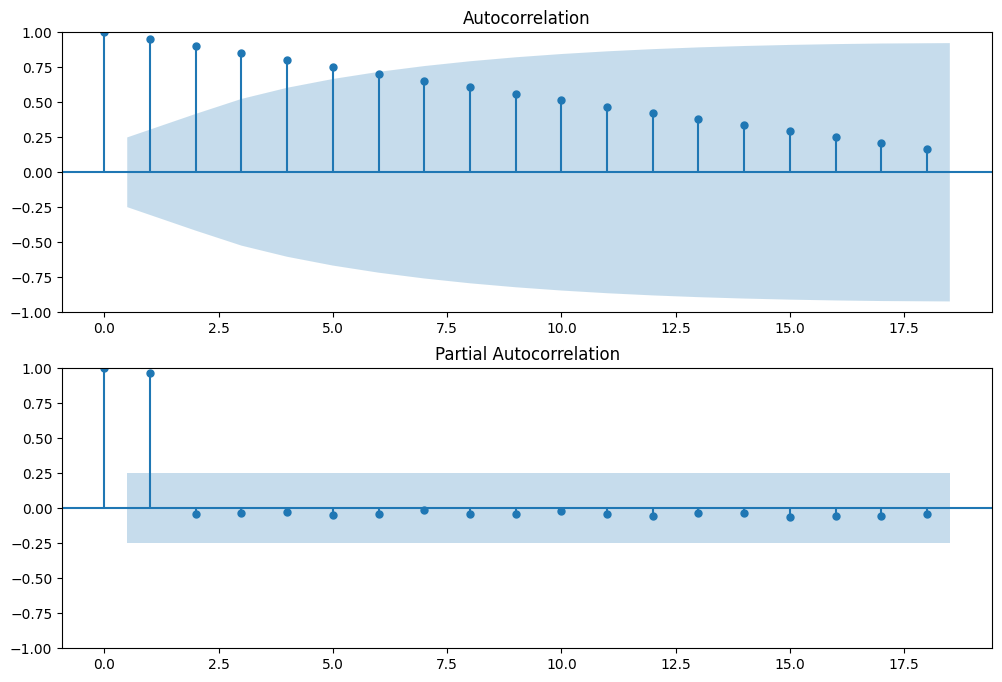
\includegraphics[scale=0.5]{pacf_acf}}
    \end{center}

    For both graphs the x-axis represents lag, whereas the y-axis indicates the correlation strength. ACF graphs represent the correlation between data values that are n intervals apart. PACF graphs are similar in that they represent the same information, however they also account for the values of the intervals in between.

    The correlation that can be seen in the AFC graph is negative, indicating that large current values correspond with small values at the specified lag. The absolute correlation values represent the strength of the relationship; to construct an ARIMA model, the expected trend of these values should be random. In this case, the initial relationship between past and present values is strong, but gradually decreases over lags, indicating a clear trend of decreasing correlation strength.
    
    If the autocorrelation follows a random non-linear trend, then AR(p) and MA(q) can be applied to the graphed functions to obtain the optimal parameter values for p and q. 
    However, this is only assuming the data does not have a trend or seasonality component, which does not apply to the given dataset.
    
    The autocorrelation trend as well as the high order of differencing required to transform the data to stationary (as seen in the ADF test) both demonstrate that the given dataset is unsuitable for constructing an ARIMA model, and therefore this prediction model has been rejected and will not be used as part of the predicted CO\textsubscript{2} and temperature values.
    

    \section{Evaluation}
    To rank the 4 accepted predictive models on their mathematical accuracy, the following error metrics are to be calculated for each model and then compared with each other:

    --------------ANOTHER TABLE---------------------------

    \subsection{Separation of Known Values into Testing and Training data}
    75\% of known data values are allocated to the testing data group, remaining 25\% are allocated to the training group. The predictive model will take in the training group data values as its sole input, and will predict the remaining 25\%. The model’s predicted values are then to be compared with the training group’s values and the forecast errors obtained.
    A forecast error is defined as the difference between an observed and its forecasted value; the formula for a single forecast error can be modified to suit multiple data values, and it is denoted by the following equation:
    
    ${e_{T+h} = y_{T+h} - \hat{y}_{T+h|T}}$
    
    Where:
    \begin{itemize}
        \item ${e_{T+h}}$ = Forecast error 
        \item ${y_{T+h}}$ = Actual value of the h-step observation
        \item ${\hat{y}_{T+h|T}}$ = Actual value of the h-step forecast
    \end{itemize}
    
    
    [ADD GRAPHED RESULTS HERE + CALCULATED FORECAST ERRORS]
    
    It is important to note that although a model may fit the training data well, it does not necessarily mean the model will forecast well, therefore it is important to take the other error metrics into consideration.

    \subsection{MSE}
    Mean Squared Error (MSE) is a measure of the quality of a predictor or of an assessor, its definition differing accordingly. It is the average squared distance between the actual and predicted values, measuring the variance of the residuals. In this case, only the quality of the predictor is to be assessed. It involves taking the average squared distance between the actual and predicted values, measuring the variance of the residuals. The within-sample MSE of a predictor can then be denoted as:

    ${\operatorname {MSE} ={\frac {1}{n}}\sum _{i=1}^{n}\left(Y_{i}-{\hat {Y_{i}}}\right)^{2}}$
    
    Where:
    \begin{itemize}
        \item ${\frac {1}{n}\sum _{i=1}^{n}}$ = Mean
        \item ${\left(Y_{i}-{\hat {Y_{i}}}\right)^{2}}$ = Squares of the errors
    \end{itemize}
    
     MSE also has a differentiable graph so it makes it easier to perform mathematical operations in comparison to MAE. MSE is more sensitive to outliers compared to MAE. 

    \subsection{RMSE}
    Root Mean Squared Error (RMSE) is the square root of the MSE, measuring the standard deviation of the residuals. The higher the RMSE value, the larger the deviation between actual and predicted values. By proxy, the lower the RMSE value, the lower the deviation, hence the model is more accurate. Building on the last error metric formula, RMSE can be denoted as:
    
    ${\operatorname {RMSE} = \sqrt{MSE}}$
    
    When outliers are exponentially rare, such as this situation, RMSE is generally preferred over MSE as it provides a better evaluation of model performance, as it uses the same units as the Y axis (CO\textsubscript{2} emissions).

    \subsection{MAE}
    Mean Absolute Error (MAE) is the sum of the absolute difference between the actual and predicted values. A perfect prediction model would yield a 0 as its MAE value. The further away from 0 the MAE value is, the more errors the model makes and hence the less accurate the model is. The formula to calculate MAE is denoted as:

    ${\displaystyle {MAE} ={\frac {\sum _{i=1}^{n}\left|y_{i}-x_{i}\right|}{n}}}$
    
    Where:
    \begin{itemize}
        \item ${\sum _{i=1}^{n}\left|y_{i}-x_{i}\right|}$ = Sum of absolute error
        \item {n} = Number of errors
    \end{itemize}

    \subsection{PMCC, ${R^2}$ AND COVARIANCE}
    The last 3 error metrics are explained in further detail when exploring the relationship between temperature and CO\textsubscript{2} emissions

    \subsection{Results}
    The MSE, RMSE, MAE, PMCC, R^2 and covariance were calculated for each accepted model, rounded to 5 s.f, and compiled into a results table below. For each error metric, the model with the value closest to and furthest from a perfect value were highlighted:

    ---------------A TABLE, AGAIN.-------------------
    --------------LO AND BEHOLD, ANOTHER TABLE--------------



    \section{Model Analysis}

    \subsection{Parameter Sensitivity}
    blah blah

    \subsection{General Evaluation}

    \noindent\textbf{Strength 1}: asdf

    \noindent\textbf{Strength 2}: asdf

    \noindent\textbf{Weakness 1}: asdf

    \subsection{Possible Improvements}
    blah blah


    \newpage


    \section{References}

    \subsection{Program Code}
    \noindent Result data generated:
    \begin{verbatim}
    text data stuff

    \end{verbatim}

    \noindent Python program code:
    \begin{lstlisting}[language=Python]
        # pass

    \end{lstlisting}

    \subsection{Bibliography}
%    \printbibliography

\end{document}
